\documentclass[12pt]{article}

\usepackage[utf8]{inputenc}
\usepackage[T1]{fontenc}
\usepackage[french]{babel}
\usepackage[a4paper, margin=2cm]{geometry}
\usepackage{wrapfig}

\usepackage{qtree}
\usepackage{tikz}
\usepackage{tikz-qtree}



\usepackage{listings}
\usepackage{color}
\definecolor{dkgreen}{rgb}{0,0.6,0}
\definecolor{gray}{rgb}{0.5,0.5,0.5}
\definecolor{mauve}{rgb}{0.58,0,0.82}
\definecolor{Darkblue}{rgb}{0,0,0.5}


\usepackage{hyperref}
\hypersetup{
    colorlinks=true,
    linkcolor=Darkblue,
    filecolor=magenta,      
    urlcolor=cyan,
    pdfpagemode=FullScreen,
    }

\lstset{frame=tb,
  language=C,
  aboveskip=3mm,
  belowskip=3mm,
  showstringspaces=false,
  columns=flexible,
  basicstyle={\small\ttfamily},
  numbers=none,
  numberstyle=\tiny\color{gray},
  keywordstyle=\color{blue},
  commentstyle=\color{dkgreen},
  stringstyle=\color{mauve},
  breaklines=true,
  breakatwhitespace=true,
  tabsize=3,
  numbers=left,
  numbersep=10pt
}


\usepackage{fancyhdr}
\pagestyle{fancy}
\renewcommand{\headrulewidth}{0pt}
\fancyhead[C]{} 
\fancyhead[L]{}
\fancyhead[R]{}

\renewcommand{\footrulewidth}{1pt}
\fancyfoot[C]{Outils d'Aide à la Décision - TP 3\\\textbf{Page \thepage/\pageref{lastPage}}}
\fancyfoot[L]{Ao XIE \\ Chloé BERTHOLD}
\fancyfoot[R]{ISIMA}


\usepackage{array,multirow,makecell}
\setcellgapes{1pt}
\makegapedcells
\newcolumntype{R}[1]{>{\raggedleft\arraybackslash }b{#1}}
\newcolumntype{L}[1]{>{\raggedright\arraybackslash }b{#1}}
\newcolumntype{C}[1]{>{\centering\arraybackslash }b{#1}}




\begin{document}
    \def\arraystretch{1.5}
    
        
\includegraphics[scale = 0.8]{Photos/isima.jpg}  
        \hfill
        \begin{large}
            Enseignant : Philippe LACOMME
        \end{large}
        
    \vspace{5cm}
    \begin{center}
        \begin{Huge}
            \textbf{Outils d'Aide à la Décision ZZ2 - TP 3}
            \\
            \vspace{0.3cm}
            \textbf{Vehicle Routing Problem}
        \end{Huge}
    \end{center}
    
    \begin{center}
        \begin{large}
            Ao XIE \& Chloé BERTHOLD - Décembre 2022
        \end{large}
    \end{center}
    
    \vspace{3cm}
	\begin{center}
	    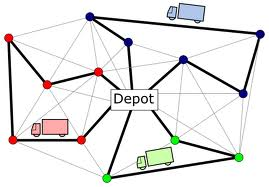
\includegraphics[scale=1]{Photos/vrp.jpg}
	\end{center}
    \thispagestyle{empty}
    \newpage
    \begin{center}
    \section*{Introduction}    
    \end{center}
    \par
    Le problème du trajet du véhicule est un problème d'optimisation intégrative, qui est très étudié dans le domaine de l'optimisation combinatoire discrète et qui a de nombreuses applications dans le secteur de la logistique. Ce problème peut être résolu en optimisant le trajet du véhicule, ce qui permet de réduire efficacement les coûts de logistique et de distribution. Parallèlement, ce problème a été proposé pour la première fois par Dantzig et Ramser en 1959, et se réfère à un certain nombre de clients, chacun ayant un nombre différent de biens en demande, auxquels un centre de distribution fournit des biens et une flotte de véhicules est chargée de distribuer les biens et d'organiser des itinéraires appropriés, dans le but de satisfaire les besoins du client et d'atteindre, sous certaines contraintes, des objectifs tels que la distance la plus courte, le moindre coût et le moindre temps passé.
    \par
    En 1986, EK Baker et JR Schaffer et al. ont proposé le problème de l'ordonnancement des véhicules avec des contraintes de fenêtre temporelle\cite{baker1986solution}, auquel plusieurs niveaux de complexité différents ont été ajoutés. En 1999, Gulay Barbarosoglu et al. ont développé une nouvelle heuristique de recherche tabou\cite{barbarosoglu1999tabu}. Une nouvelle procédure de génération de voisinage a été proposée, qui tient compte des modèles de diffusion aux emplacements des distributeurs. En 2006, J. Brandao et al. ont publié un nouvel algorithme de recherche d'étiquettes pour le problème de l'acheminement des véhicules de collecte\cite{brandao2006new}, transformant le problème $vehicle$ $routing$ $problem(VRP)$ en un problème $vehicle$ $routing$ $problem$ $with$ $backhauls(VRPB)$ et proposant une solution. Et lorsque nous revenons à un futur proche, en 2022, Carmine Cerrone et Anna Sciomachen et al. se concentrent sur le problème VRP dans une perspective de mobilité intelligente, avec pour objectif de minimiser les composantes de coût de l'itinéraire\cite{cerrone2022vrp}, à la fois en termes de déplacement et de coûts externes dus aux questions environnementales, en fonction des véhicules choisis et des différentes rues de la ville à traverser.
    \par
    Dans cette expérience, notre objectif est de mettre en œuvre un système VRP à partir de zéro.
    
    \newpage

	\tableofcontents
	\listoffigures
	
	\newpage
	
	\section{Présentation générale}
	\subsection{Rappel des objectifs}
	Dans ce TP il est ainsi question de mettre en place un système de résolution des problèmes VRP. Pour cela, il faut implémenter des algorithmes pour la récupération d'un graphe dans un fichier, pour la génération d'un tour géant correspondant à ce graphe, pour l'évaluation de ce tour géant, pour la recherche locale et enfin une méta-heuristique pour parcourir l'espace des solutions.

	\subsection{Organisation du code source}
	Ce TP est divisé en trois fichiers :\\\par
	\begin{itemize}
	    \item Le fichier \emph{utils.h} qui regroupe les signatures de toutes les fonctions codées.
	    \item Le fichier \emph{utils.cpp} où sont implémentées les fonctions définies dans le fichier \emph{header.h}.
	    \item Le fichier \emph{tp\_vrp.cpp} qui contient la fonction main\\
	\end{itemize}\par
	 Dans les fonctions implémentées, les principales sont \emph{lire\_fichier()}, \emph{generer\_tour\_geant()}, \emph{plus\_proche\_voisin()}, \emph{autre\_heuristique()}, \emph{evaluer()}, emph{recherche\_locale()} et \emph{grasp()}. La fonction \emph{lire\_fichier()} permet de lire une structure de graphe dans un fichier et de la stocker dans une instance en paramètre, les fonctions \emph{generer\_tour\_geant()}, \emph{plus\_proche\_voisin()} et \emph{autre\_heuristique()} permettent de générer un tour géant dans le champ adapte de la structure passée en paramètre de différentes manières, la fonction \emph{evaluer()} permet d'appliquer l'algorithme split au tour géant donné, la fonction \emph{recherche\_locale()} effectue une recherche locale sur un tour géant donné et enfin la fonction \emph{grasp()} effectue une recherche dans l'espace des solutions pour trouver la solution optimale.\\\par
	 
	 \section{Fonctions de développement}
	 Ici, nous analyserons et expliquerons les points nécessaires dans la résolution d'un problème de VRP.
	 
	 \subsection{La génération d'un graphe à partir d'une séquence}
	 Pour traiter un problème de VRP, il faut être capable de générer un graphe à partir d'une séquence le décrivant. Pour cela, il faut définir une norme pour ces séquences qui soit simple à lire et à comprendre.\\\par
	 Un fichier est alors composé comme suit :\\\par
	 \begin{itemize}
	     \item Une première ligne ne contenant que le nombre de clients à traiter.
          \item Une deuxième ligne concernant les véhicule avec le nombre de véhicules et leur capacité.
	     \item Une série de $n$ lignes où $n$ est le nombre de clients. Chaque ligne se compose de distances entre le sommet $i$ où i est le numéro de la ligne et le sommet $j$ où j est le numéro de la ligne plus le numéro de la colonne. Les distances entre $i$ et $j$ étant symétriques, on peut ne garder que la partie supérieure du tableau symétrique.\\
         \item Une dernière série de $n$ ligne où chaque ligne se compose uniquement de la demande du client $i$ où i est le numéro de la ligne.
	 \end{itemize}\par

  \begin{figure}[!h]
	    \centering
	    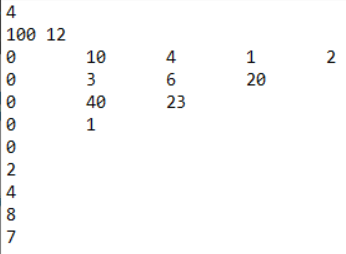
\includegraphics[scale = 1]{fichier.png}
	    \caption{Exemple d'un fichier}
	    \label{fig1}
	\end{figure}\par
	 La fonction \emph{lire\_fichier()} permet de convertir ces séquences en un graphe.

    \subsection{La génération d'un tour géant}
    Pour évaluer une solution, il faut tout d'abord générer un tour géant. Pour cela, trois choix sont possibles.
    \subsubsection{Le plus proche voisin}
        Ici, le tour géant est généré en prenant à chaque fois le plus proche voisin en terme de distance. En partant du sommet 0, le dépôt, on observe les distances entre le sommet considéré et tous les autres sommets et on insère le plus proche dans la séquence du tour géant.
         \begin{figure}[!h]
	    \centering
	    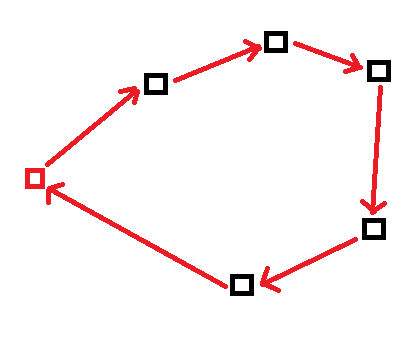
\includegraphics[scale = 1]{plu_proche.png}
	    \caption{Exemple de la création d'un tour géant avec la méthode du plus proche voisin}
	    \label{fig2}
	\end{figure}\par

 \subsubsection{Le plus proche voisin randomisé}
    Ici, on applique sensiblement la même méthode mais en ajoutant du hasard. Pour chaque nouveau sommet (en commençant par le dépôt), on récupère les quatre plus proche voisins que l'on ordonne du plus proche au plus éloigné. Puis on fait un tirage. On a alors 80\% de chance de prendre le premier voisin, c'est à dire le plus proche. Si on tombe dans les 20\% restants, on refait un tirage avec le même pourcentage de chance pour le deuxième plus proche, et ainsi de suite jusqu'à soit arriver au dernier voisin, soit faire un bon tirage.
     \begin{figure}[!h]
	    \centering
	    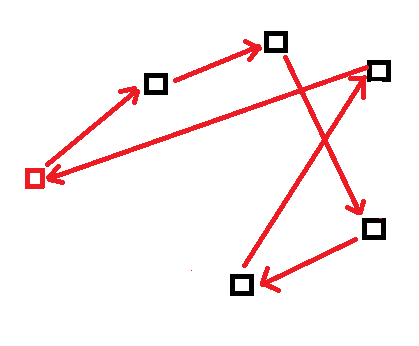
\includegraphics[scale = 1]{plu_proche_rand.png}
	    \caption{Exemple de la création d'un tour géant avec la méthode du plus proche voisin randomisé}
	    \label{fig3}
	\end{figure}\par

 \subsubsection{Autre méthode}
 La dernière méthode consiste à s'éloigner le plus possible du dépôt au départ puis d'y revenir une fois que l'on a traité au moins la moitié de la demande totale. Pour chaque sommet, on récupère une nouvelle fois les quatre plus proche voisins, mais cette fois-ci, on sélectionne celui qui s'éloigne le plus du dépôt, c'est à dire qui a la distance la plus élevée avec le dépôt. Une fois que la demande cumulée des clients traité dépasse la moitié de la demande totale, on sélectionne le voisin qui se rapproche le plus du dépôt, c'est à dire qui a la plus faible distance avec le dépôt.
 \begin{figure}[!h]
	    \centering
	    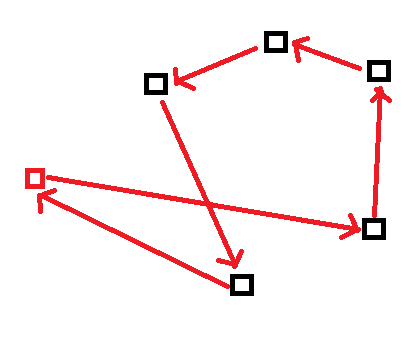
\includegraphics[scale = 1]{autre.png}
	    \caption{Exemple de la création d'un tour géant avec la dernière méthode}
	    \label{fig4}
	\end{figure}\par
  
	 \subsection{L'évaluation du graphe}
	 \hypertarget{eval}{}
	 \subsubsection{Principe}
	 L'évaluation d'une solution se base sur l'algorithme de SPLIT. On suppose que la flotte de véhicules est infinie. L'algorithme va donc parcourir les clients jusqu'à avoir dépassé la capacité du véhicule puis prendre un nouveau véhicule pour parcourir les suivants. A la fin de l'algorithme, les clients seront divisés en plusieurs tournées.
    \begin{figure}[!h]
	    \centering
	    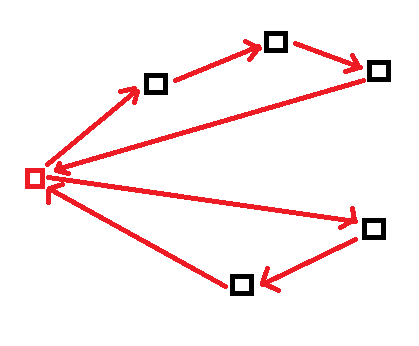
\includegraphics[scale = 1]{split.png}
	    \caption{Exemple du résultat du SPLIT sur un tour géant généré à l'aide de la méthode du plus proche voisin}
	    \label{fig5}
	\end{figure}\par
	 
	 \subsubsection{La procédure \emph{evaluer()}}\hypertarget{evaluer}{}
	 La fonction \emph{evaluer()} permet de calculer les dates d'arrivée du véhicule pour tous les clients ainsi que leur père dans les champs de la structure de solution passée en paramètre par rapport au graphe donné en paramètre et à un tour géant déterminé à l’avance.\\\par
	 
	\subsection{La recherche locale}
	\subsubsection{Principe}
	Ne calculer qu'une solution n'est pas très efficace, on a de grandes chances de tomber sur un coût très élevé alors qu'il existe de bien meilleures solutions. C'est pourquoi il est important d'effectuer une recherche locale : une fois une solution sélectionnée, on s'en sert pour descendre le plus possible et aller chercher un minimum local. Il est crucial que cette recherche locale soit efficace car elle sera ensuite utilisée énormément de fois pour trouver le minimum global.\\\par
	Elle est ici effectuée à partir de quatre mouvements, tirés aléatoirement à chaque itération :\\
 \begin{itemize}
     \item Le re-insert, qui consiste à déplacer un sommet dans la tournée de sorte à réduire le détour nécessaire pour y accéder et en repartir.
     \item Le re-insert double, qui est le frère du re-insert mais qui permet d'essayer d'insérer le sommet dans une deuxième tournée.
     \item Le 2-opt, qui va inverser une partie de la tournée.
     \item Le 2-opt inter-tournée, qui tente de croiser une partie d'une tournée avec une partie d'une autre tournée.
 \end{itemize}
	\subsubsection{La procédure \emph{recherche\_locale()}}\hypertarget{recherche}{}
	 La fonction \emph{recherche\_locale()} permet de réaliser une amélioration de type descente à partir d’une première solution calculée grâce au tour géant renseigné dans la structure de solution donnée en paramètre.\par
	 A chaque nouvelle itération, on tire avec une certaine probabilité un des quatre mouvement que l'on applique à une ou deux tournées. Puis, on récupère le tour géant correspondant à cette modification et on évalue à nouveau le graphe. Si la solution trouvée est meilleur que la précédente, on augmente la probabilité de choisir le mouvement, sinon on la baisse.
	
	\subsection{La méta-euristique}\hypertarget{grasp}{}
	\subsubsection{Principe}
	La recherche locale permet d'obtenir un coût final beaucoup plus satisfaisant qu'une simple évaluation, cependant elle ne donne qu'un minimum local et pas le minimum global. C'est pourquoi il est nécessaire de mettre en place un algorithme qui va chercher le minimum global, ici l'algorithme Grasp. Pour cela, on cherche un minimum local à partir duquel on génère un certain nombre de voisins (permutations aléatoires du tour géant) pour parcourir l'espace et découvrir de nouveau minimum locaux, en mémorisant toujours la meilleure solution.
	\subsubsection{La procédure \emph{grasp()}}
	\emph{Greedy Random Adaptive Search Procedure }(GRASP) est une métathéorique, Il s'agit d'un algorithme d'optimisation classique et efficace. Pour cela, on crée un tour géant (de l'une des trois façons présentées) à partir duquel on effectue une recherche locale pour chercher le minimum local. A partir de cette solution, on crée plusieurs solutions voisines en permutant simplement les clients dans le tour géant et on leur applique aussi la recherche locale pour trouver d'autres minimums locaux. On garde toujours la meilleure solution. On effectue la recherche de solutions voisines un certains nombres de fois puis on change complètement de tour géant pour explorer une autre partie de l'espace des solution auquel on applique le même traitement.\\\par
    A la fin de l'algorithme, l'espace des solutions aura été balayé efficacement et on aura trouvé la solution optimale, ou du moins une solution qui s'en rapproche grandement.
	
	\section{Étude de séquence}
	Nous allons à présent mettre les algorithmes à l'épreuve sur une séquence, celle de Paris et étudier les résultats.\par
	\subsection{Évaluation simple}
	Comme expliqué \hyperlink{eval}{plus haut}, n'évaluer qu'une seule fois une solution n'est pas très efficace et peut donner des résultats très insatisfaisants.\\\par
	L'application de l'algorithme SPLIT sur la séquence de Paris donne le résultat suivant :\\\par
        \begin{figure}[!h]
	    \centering
	    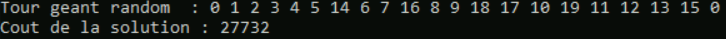
\includegraphics[scale = 1]{res_eval.png}
	    \caption{Résultat de SPLIT sur la séquence de Paris avec un tour géant généré avec la méthode du plus proche voisin randomisé}
	    \label{fig6}
	\end{figure}\par
	\newpage
	\subsection{Recherche locale}
	La recherche locale permet de trouver un minimum local et donc d'obtenir des résultats beaucoup plus intéressants. Appliquée à la séquence de Paris, le coût total est le suivant :\\\par
    \begin{figure}[!h]
	    \centering
	    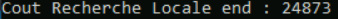
\includegraphics[scale = 1]{local.png}
	    \caption{Résultat de la recherche locale appliquée à la séquence de Paris}
	    \label{fig7}
	\end{figure}\par
    On remarque bien que le coût total a baissé mais on peut intuiter que ce n'est pas suffisant, c'est pourquoi il faut utiliser un algorithme tel que le GRASP pour se rapprocher de la solution optimale.
	
    \subsection{Grasp}
    Grâce à l'algorithme de GRASP, on peut se rapprocher de la solution optimale et donc réduire grandement les coûts. Appliqué à la séquence de Paris, on trouve le coût final suivant :
    \begin{figure}[!h]
	    \centering
	    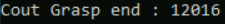
\includegraphics[scale = 1]{grasp.png}
	    \caption{Résultat de l'algorithme de GRASP appliqué à la séquence de Paris}
	    \label{fig8}
	\end{figure}\par
    \section{Conclusion}
    Dans ce TP, il était question d'implémenter les algorithmes nécessaires à la résolution d'un problème de routing de véhicules. La difficulté du problème réside dans la recherche locale qui s'appuie sur quatre mouvements différents. Pour ce genre de problème, il est nécessaire d'appliquer un algorithme tel que celui du GRASP pour espérer se rapprocher d'une solution optimale.
 
    \newpage	    
    \bibliographystyle{ieeetr}
    \bibliography{réf}
	\label{lastPage}
	    
	    

\end{document}